%% LyX 2.0.3 created this file.  For more info, see http://www.lyx.org/.
%% Do not edit unless you really know what you are doing.
\documentclass[10pt]{beamer}\usepackage[]{graphicx}\usepackage[]{color}
%% maxwidth is the original width if it is less than linewidth
%% otherwise use linewidth (to make sure the graphics do not exceed the margin)
\makeatletter
\def\maxwidth{ %
  \ifdim\Gin@nat@width>\linewidth
    \linewidth
  \else
    \Gin@nat@width
  \fi
}
\makeatother

\definecolor{fgcolor}{rgb}{0.345, 0.345, 0.345}
\newcommand{\hlnum}[1]{\textcolor[rgb]{0.686,0.059,0.569}{#1}}%
\newcommand{\hlstr}[1]{\textcolor[rgb]{0.192,0.494,0.8}{#1}}%
\newcommand{\hlcom}[1]{\textcolor[rgb]{0.678,0.584,0.686}{\textit{#1}}}%
\newcommand{\hlopt}[1]{\textcolor[rgb]{0,0,0}{#1}}%
\newcommand{\hlstd}[1]{\textcolor[rgb]{0.345,0.345,0.345}{#1}}%
\newcommand{\hlkwa}[1]{\textcolor[rgb]{0.161,0.373,0.58}{\textbf{#1}}}%
\newcommand{\hlkwb}[1]{\textcolor[rgb]{0.69,0.353,0.396}{#1}}%
\newcommand{\hlkwc}[1]{\textcolor[rgb]{0.333,0.667,0.333}{#1}}%
\newcommand{\hlkwd}[1]{\textcolor[rgb]{0.737,0.353,0.396}{\textbf{#1}}}%
\newcommand\myeq{\stackrel{\mathclap{\normalfont\mbox{d}}}{=}}




\usepackage{fontawesome5}
\usepackage{framed}
\makeatletter
\newenvironment{kframe}{%
 \def\at@end@of@kframe{}%
 \ifinner\ifhmode%
  \def\at@end@of@kframe{\end{minipage}}%
  \begin{minipage}{\columnwidth}%
 \fi\fi%
 \def\FrameCommand##1{\hskip\@totalleftmargin \hskip-\fboxsep
 \colorbox{shadecolor}{##1}\hskip-\fboxsep
     % There is no \\@totalrightmargin, so:
     \hskip-\linewidth \hskip-\@totalleftmargin \hskip\columnwidth}%
 \MakeFramed {\advance\hsize-\width
   \@totalleftmargin\z@ \linewidth\hsize
   \@setminipage}}%
 {\par\unskip\endMakeFramed%
 \at@end@of@kframe}
\makeatother

\definecolor{shadecolor}{rgb}{.97, .97, .97}
\definecolor{messagecolor}{rgb}{0, 0, 0}
\definecolor{warningcolor}{rgb}{1, 0, 1}
\definecolor{errorcolor}{rgb}{1, 0, 0}
\newenvironment{knitrout}{}{} % an empty environment to be redefined in TeX

\usepackage{alltt}
\usepackage[T1]{fontenc}
\setcounter{secnumdepth}{3}
\setcounter{tocdepth}{3}
\usepackage{tikz}
\usepackage{color}
\usepackage{colortbl}
\usepackage{dcolumn}
\usepackage{amsmath}
\usepackage{tikz}
\usepackage{floatflt}
\usepackage{multicol}
\usepackage{multirow}
\usepackage{listings}
\usepackage{tabularx}
\usepackage{amssymb}% http://ctan.org/pkg/amssymb
\usepackage{pifont}% http://ctan.org/pkg/pifont
\usepackage{bbm}
\usepackage{siunitx}
\usepackage{url}
\usepackage{verbatim}
\usepackage{enumerate}
\usepackage{algorithmic}
\usepackage{algorithm}
\usepackage[flushleft]{threeparttable}
\usepackage{algorithm}
\usepackage{amsfonts}
\usepackage{booktabs}
\usepackage{siunitx}

\usepackage{hyperref}
\hypersetup{
    colorlinks=magenta,
    linkcolor=blue,
    filecolor=magenta,      
    urlcolor=magenta
     }
     
    \definecolor{links}{HTML}{2A1B81}
\hypersetup{colorlinks,linkcolor=blue, urlcolor=magenta}


\makeatletter

%%%%%%%%%%%%%%%%%%%%%%%%%%%%%% LyX specific LaTeX commands.
\providecommand{\LyX}{\texorpdfstring%
  {L\kern-.1667em\lower.25em\hbox{Y}\kern-.125emX\@}
  {LyX}}


%%%%%%%%%%%%%%%%%%%%%%%%%%%%%% Textclass specific LaTeX commands.
 % this default might be overridden by plain title style
 \newcommand\makebeamertitle{\frame{\maketitle}}%
 \AtBeginDocument{
   \let\origtableofcontents=\tableofcontents
   \def\tableofcontents{\@ifnextchar[{\origtableofcontents}{\gobbletableofcontents}}
   \def\gobbletableofcontents#1{\origtableofcontents}
 }
 \def\lyxframeend{} % In case there is a superfluous frame end
 \long\def\lyxframe#1{\@lyxframe#1\@lyxframestop}%
 \def\@lyxframe{\@ifnextchar<{\@@lyxframe}{\@@lyxframe<*>}}%
 \def\@@lyxframe<#1>{\@ifnextchar[{\@@@lyxframe<#1>}{\@@@lyxframe<#1>[]}}
 \def\@@@lyxframe<#1>[{\@ifnextchar<{\@@@@@lyxframe<#1>[}{\@@@@lyxframe<#1>[<*>][}}
 \def\@@@@@lyxframe<#1>[#2]{\@ifnextchar[{\@@@@lyxframe<#1>[#2]}{\@@@@lyxframe<#1>[#2][]}}
 \long\def\@@@@lyxframe<#1>[#2][#3]#4\@lyxframestop#5\lyxframeend{%
   \frame<#1>[#2][#3]{\frametitle{#4}#5}}

\renewcommand{\footnotesize}{\fontsize{6pt}{6pt}\selectfont}


\newcommand{\indep}{\rotatebox[origin=c]{90}{$\models$}}

% https://dkumor.com/posts/technical/2018/08/15/causal-tikz/

% Tikz settings optimized for causal graphs.
% Just copy-paste this part
\usetikzlibrary{shapes,decorations,arrows,calc,arrows.meta,fit,positioning}
\tikzset{
    -Latex,auto,node distance =1 cm and 1 cm,semithick,
    state/.style ={ellipse, draw, minimum width = 0.7 cm},
    point/.style = {circle, draw, inner sep=0.04cm,fill,node contents={}},
    bidirected/.style={Latex-Latex,dashed},
    el/.style = {inner sep=2pt, align=left, sloped}
}


%%%%%%%%%%%%%%%%%%%%%%%%%%%%%% User specified LaTeX commands.
%\usetheme{Warsaw}
\usetheme{Boadilla}
%\setbeamertemplate{navigation symbols}{}
%gets rid of bottom navigation bars
%\setbeamertemplate{footline}[page number]{}
%\setcounter{page}{44}
%\setbeamertemplate{footline}{}


\makeatother
\IfFileExists{upquote.sty}{\usepackage{upquote}}{}

\begin{document}


\title[Personalization with Latent Confounders]{Personalized Marketing with Latent Confounders}
\author[Leo Guelman]{Leo Guelman}
\institute[RBC Royal Bank]{RBC Royal Bank}
\date[December 2022]
{}
\makebeamertitle

\lyxframeend{}


%%%%Slide

\begin{frame}
[fragile]\frametitle{Inspiration for Personalized Marketing}

% This is Ronald Fisher, he was a statistician and probably one of the most relevant figures in 20th century statistics 
% He's been probably most famous for his contribution to experimental design (a.k.a. A/B testing).
% He was the first to propose randomization in experiments as mechanism to eliminate confounding bias, and be able to disentangle causal relationships
% To this day A/B testing (or RCTs in clinical trials) is considered the Gold Standard to learn causal relationships in Clinical Trials and Marketing.

%\begin{figure}[t]
%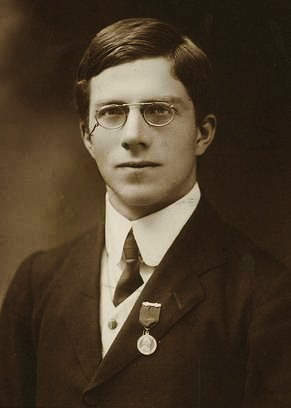
\includegraphics[width=3cm]{figures/fisher.jpg}
%\caption{Ronald Fisher (1890-1962)}
%\centering
%\end{figure}



\begin{columns}[T] % align columns
\begin{column}{.48\textwidth}

\vskip25pt

\small{

\begin{itemize}

\item Personalization is founded on the premise that individuals have heterogenous response to actions.
% the optimal action for person A and person B might be different. 

\vskip7pt

\item Personalization algorithms aim to improve decision-making by identifying and exploiting this heterogeneity.

\end{itemize}
}


\end{column}%
\hfill%


\begin{column}{.48\textwidth}


\begin{figure}[t]
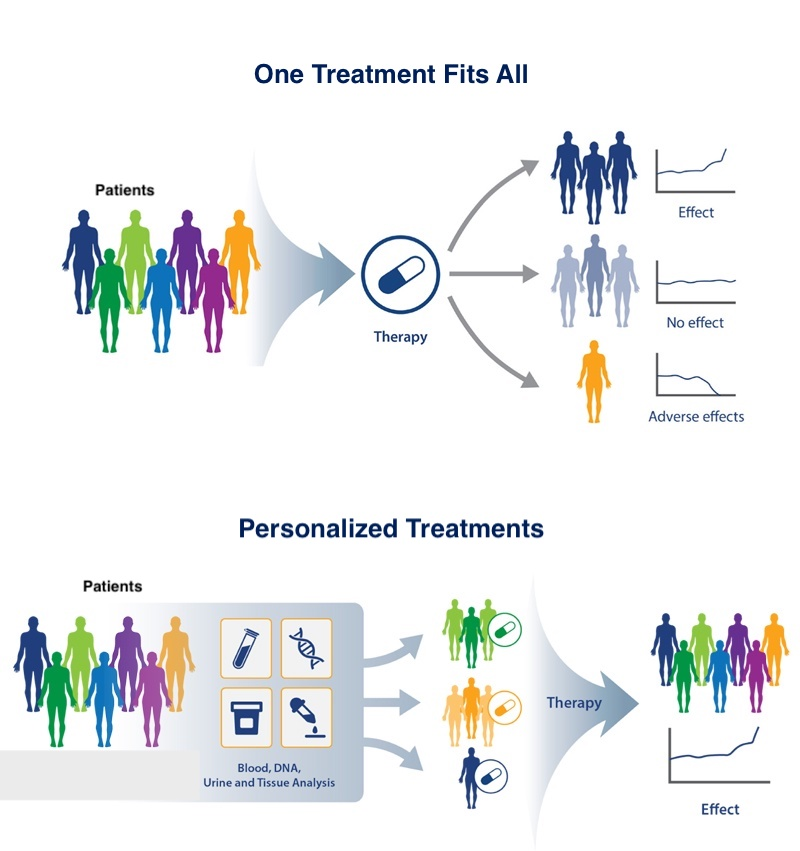
\includegraphics[width=5cm]{figures/personalizedmedv2.jpg}
\centering
\end{figure}


\end{column}%
\end{columns}


\end{frame}

%%%%Slide

\begin{frame}
[fragile]\frametitle{Estimating Treatment Effects: \textbf{Non}-Personalized Paradigm}

\small{
A/B Tests are `gold standard' in the One-Treatment-Fits-All paradigm because they remove the influence of unobserved confounders (variables that influence both the treatment and the outcome). 
}

\vskip20pt


\begin{columns}[T] % align columns
\begin{column}{.48\textwidth}

\begin{figure}[t]
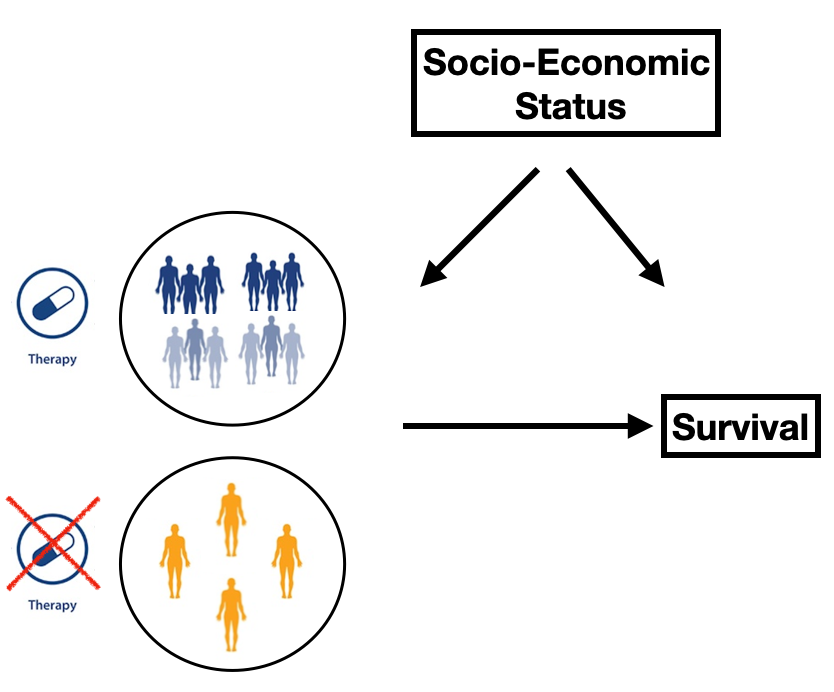
\includegraphics[width=4cm]{figures/ab1.png}
\centering
\end{figure}


\end{column}%
\hfill%

\pause

\begin{column}{.48\textwidth}

\vskip-10pt

\begin{figure}[t]
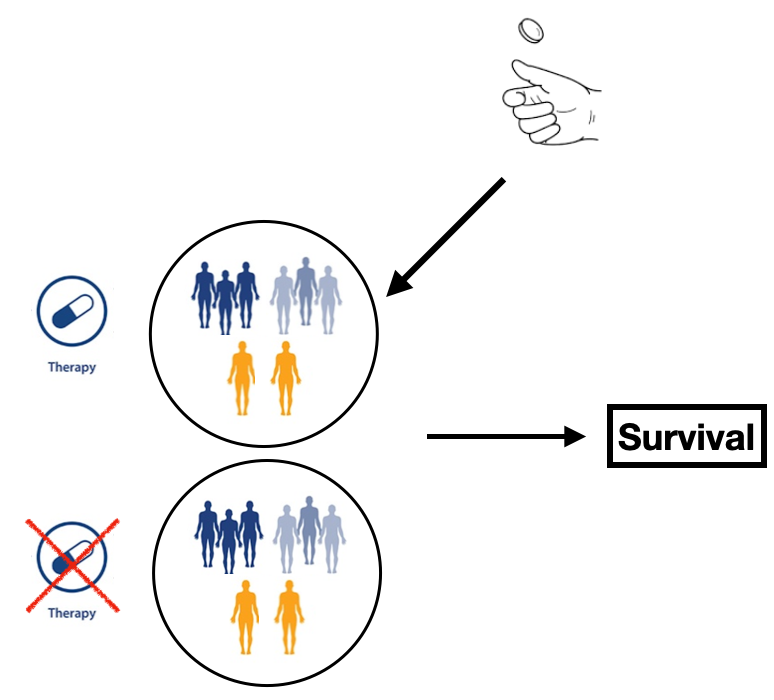
\includegraphics[width=4cm]{figures/ab2.png}
\centering
\end{figure}


\end{column}%
\end{columns}

\end{frame}

%%%%Slide

\begin{frame}
[fragile]\frametitle{Estimating Treatment Effects: Personalized Paradigm}

% If there is a singe takeaway message from what I want to talk about is that, in contrast to the idea that A/B testing should be used as the gold standard to learn causal effects, when the goal is not just to learn average treatment effects (i.e., whether a action is effective on average) but to learn personalized optimal actions, then A/B test may or may not be the best we can do.

% when the goal is to 

\begin{itemize}

\item In the presence of unobserved confounders (most plausible scenario), experimental data is likely not `gold standard' for estimating heterogenous treatment effects.

\vskip10pt

\item  A coherent fusion of experimental and observational data that results from a \emph{counterfactual}-based decision criterion is likely to outperform other approaches. 

\vskip10pt

\item In what follows, I'll use a Personalized Marketing problem as a motivating example to discuss the statements above. 

\end{itemize}

\end{frame}

%%%%Slide

\begin{frame}
[fragile]\frametitle{The Business Setting}

\begin{itemize}

\item \textbf{Business objective:}  Sell a credit card to new-to-RBC clients. 


\item \textbf{Current campaign: One-Treatment-Fits-All paradigm}. All new-to-RBC clients who visited the RBC public site, get a credit card offer $+$ iPad incentive.


\begin{figure}
   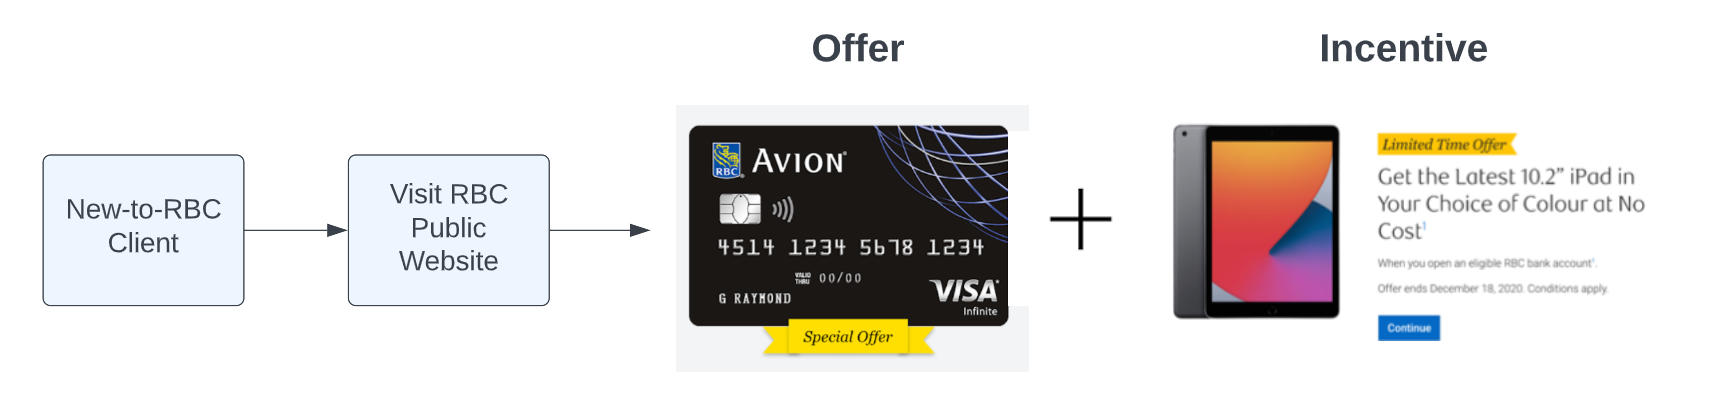
\includegraphics[width= 0.80\linewidth]{figures/campaign.png}
\end{figure}

\vskip20pt

\item \textbf{Future campaign: Personalize the incentive}. Identify which new-to-RBC clients should receive an iPad incentive in the future to maximize the expected profitability of the campaign. 

\end{itemize}

\end{frame}

%%%%Slide

\begin{frame}
[fragile]\frametitle{Data Generating Process}


\begin{columns}[T] % align columns
\begin{column}{.48\textwidth}

\begin{figure}
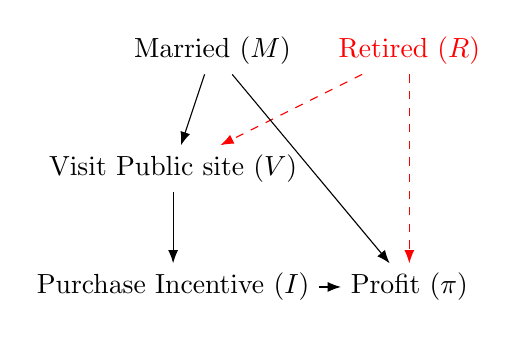
\begin{tikzpicture}
    \node (m) at (-0.5,0) {Married ($M$)};
    \node[red]  (r) at (2,0) {Retired ($R$)};
    \node (v) at (-1,-1.5) {Visit Public site ($V$)};
    \node (o) at (-1,-3) {Purchase Incentive ($I$)};
    \node (p) at (2,-3) {Profit ($\pi$)};

    \path (m) edge (v);
    \path[dashed, red] (r) edge (v);
     \path (m) edge (p);
     \path[dashed, red] (r) edge (p);
     \path (v) edge (o);
     \path (o) edge (p);
     
\end{tikzpicture}

\vskip 5pt

\caption{`True' Causal Graph (current campaign).}

\end{figure}

\end{column}%
\hfill%

\pause

\begin{column}{.48\textwidth}

\vskip 20pt

\begin{equation*}
\begin{align*}
P(m ,r)=& 0.25~\forall~m \in M, r \in R \\ 
V :=& M$\oplus$R  \\
I :=&  V 
\end{align*}
\end{equation*}
%}

\footnotesize{
\begin{table}
\begin{tabular}{ccccc}
\toprule
 &\multicolumn{2}{c}{$R=0$}
&
\multicolumn{2}{c}{$R=1$} \\\cmidrule(r){2-3}\cmidrule(l){4-5}
 & $M=1$ & $M=0$     & $M=1$ & $M=0$     \\  
 \midrule
$I=1$ &  \cellcolor{blue!25}{0.25} & 0.50 & 0.45 & \cellcolor{blue!25}{0.05} \\
$I=0$ &  0.50 & \cellcolor{blue!25}{0.10} & \cellcolor{blue!25}{0.05} & 0.30 \\
\bottomrule
\end{tabular}
\vskip5pt
\caption{$E[\pi|M, R, I]$. Highlighted cells reflect (new-to-RBC) client's 'natural' choice to visit the Public site or not.}
\end{table}
}


\end{column}%
\end{columns}
\end{frame}

%%%%Slide

\begin{frame}
[fragile]\frametitle{Approach 1: Empirical Decision Criterion (EDC)}

\begin{columns}[T] % align columns
\begin{column}{.48\textwidth}

\begin{center}
EDC  $\rightarrow$ $\underset{I \in {0,1}}{\mathrm{argmax}}~E[\pi|I, M]$
\end{center}

\vskip10pt


\begin{equation*}
\begin{align*}
E[\pi | I=1, M=1] =& 0.25\\
E[\pi | I=0, M=1] =& 0.05\\
E[\pi | I=1, M=0] =& 0.05\\
E[\pi | I=0, M=0] =& 0.10 \\
\end{align*}
\end{equation*}


\end{column}%
\hfill%


\begin{column}{.48\textwidth}

\vskip 30pt

\footnotesize{
\begin{table}
 \begin{tabular}{ccccc}
\toprule
 &\multicolumn{2}{c}{$R=0$}
&
\multicolumn{2}{c}{$R=1$} \\\cmidrule(r){2-3}\cmidrule(l){4-5}
 & $M=1$ & $M=0$     & $M=1$ & $M=0$     \\  
 \midrule
$I=1$ &  \cellcolor{blue!25}{0.25} & 0.50 & 0.45 & \cellcolor{blue!25}{0.05} \\
$I=0$ &  0.50 & \cellcolor{blue!25}{0.10} & \cellcolor{blue!25}{0.05} & 0.30 \\
\bottomrule
\end{tabular}
\vskip5pt
\caption{$E[\pi|M, R, I]$.}
\end{table}
}



\end{column}%
\end{columns}

\vskip15pt

\pause

\textbf{Decision Rule}:

\small{
\begin{itemize}
\item If Visit Site $\land$ Married $\rightarrow$ Purchase Incentive $\rightarrow~E[\pi] = \textbf{0.25}  $
\item If Visit Site $\land$ Not Married $\rightarrow$ No Purchase Incentive  $\rightarrow~E[\pi] = \textbf{0.30} $
\end{itemize}
}

\vskip10pt

Expected profit = $\boxed{\mathbf{0.275}}$ = (0.25+0.30)/2.



\end{frame}


%%%%Slide

\begin{frame}
[fragile]\frametitle{Approach 2: Post-Visit Randomization (PVR)}

\begin{columns}[T] % align columns
\begin{column}{.48\textwidth}

\begin{figure}
\begin{tikzpicture}[thick,scale=0.8, every node/.style={scale=0.8}]
    \node (m) at (-0.5,0) {Married ($M$)};
    \node[red]  (r) at (2,0) {Retired ($R$)};
    \node (v) at (-1,-1.5) {Visit Public site ($V$)};
    \node (o) at (-1,-3) {Purchase Incentive ($I$)};
    \node (p) at (2,-3) {Profit ($\pi$)};
    \node[blue] (c)  at (-4,-1.5) {Coin Flip ($C$)};

    \path (m) edge (v);
    \path[dashed, red] (r) edge (v);
     \path (m) edge (p);
     \path[dashed, red] (r) edge (p);
     \path (v) edge (o);
     \path (o) edge (p);
     \path[blue] (c) edge (o)
     
\end{tikzpicture}

\vskip 5pt

\caption{Causal DAG with post-visit randomization.}

\end{figure}

\end{column}%

\begin{column}{.48\textwidth}


\vskip 20pt

\begin{equation*}
\begin{align*}
V :=& M~$\oplus{}$ R  \\
I :=&  V \textcolor{blue}{\land C} 
\end{align*}
\end{equation*}


\end{column}%
\end{columns}

\end{frame}


%%%%Slide

\begin{frame}
[fragile]\frametitle{Approach 2: Post-Visit Randomization (PVR) - cont'd}


\begin{columns}[T] % align columns
\begin{column}{.48\textwidth}

\begin{center}
PVR $\rightarrow$ $\underset{I \in {0,1}}{\mathrm{argmax}}~E[\pi| do(I), M, V=1]$
\end{center}

\vskip10pt


\begin{equation*}
\begin{align*}
E[\pi | do(I=1), M=1, V=1] =& 0.25\\
E[\pi | do(I=0), M=1, V=1] =& 0.50\\
E[\pi | do(I=1), M=0, V=1] =& 0.05\\
E[\pi | do(I=0), M=0, V=1] =& 0.30
\end{align*}
\end{equation*}


\end{column}%
\hfill%


\begin{column}{.48\textwidth}

\vskip 30pt

\footnotesize{
\begin{table}
 \begin{tabular}{ccccc}
\toprule
 &\multicolumn{2}{c}{$R=0$}
&
\multicolumn{2}{c}{$R=1$} \\\cmidrule(r){2-3}\cmidrule(l){4-5}
 & $M=1$ & $M=0$     & $M=1$ & $M=0$     \\  
 \midrule
$I=1$ &  \cellcolor{blue!25}{0.25} & 0.50 & 0.45 & \cellcolor{blue!25}{0.05} \\
$I=0$ &  0.50 & \cellcolor{blue!25}{0.10} & \cellcolor{blue!25}{0.05} & 0.30 \\
\bottomrule
\end{tabular}
\vskip5pt
\caption{$E[\pi|M, R, I]$.}
\end{table}
}



\end{column}%
\end{columns}

\vskip15pt

\pause


\textbf{Decision Rule}:

\small{
\begin{itemize}
\item If Visit Site $\land$ Married $\rightarrow$ No Purchase Incentive $\rightarrow~E[\pi] = \textbf{0.50} $
\item If Visit Site $\land$ Not Married $\rightarrow$ No Purchase Incentive  $\rightarrow~E[\pi] = \textbf{0.30} $
\end{itemize}
}

\vskip10pt

Expected profit = $\boxed{\mathbf{0.40}}$ = (0.50+0.30)/2.



\end{frame}

%%%%Slide


\begin{frame}
[fragile]\frametitle{Approach 3: A/B Test on All New-to-RBC Clients}

\begin{columns}[T] % align columns
\begin{column}{.48\textwidth}

\begin{figure}
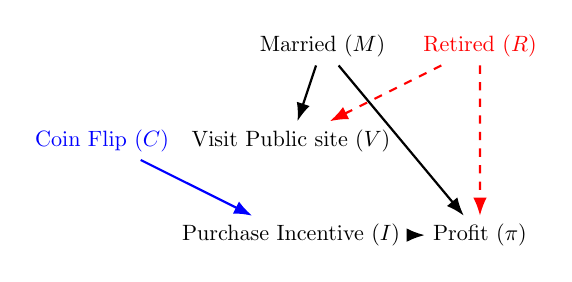
\begin{tikzpicture}[thick,scale=0.8, every node/.style={scale=0.8}]
    \node (m) at (-0.5,0) {Married ($M$)};
    \node[red]  (r) at (2,0) {Retired ($R$)};
    \node (v) at (-1,-1.5) {Visit Public site ($V$)};
    \node (o) at (-1,-3) {Purchase Incentive ($I$)};
    \node (p) at (2,-3) {Profit ($\pi$)};
    \node[blue] (c)  at (-4,-1.5) {Coin Flip ($C$)};

    \path (m) edge (v);
    \path[dashed, red] (r) edge (v);
     \path (m) edge (p);
     \path[dashed, red] (r) edge (p);
     \path (o) edge (p);
     \path[blue] (c) edge (o);
     
\end{tikzpicture}

\vskip 5pt


\caption{Causal DAG with A/B Test on All New-to-Bank Clients.}

\end{figure}

\end{column}%

\begin{column}{.48\textwidth}


\vskip 20pt

\begin{equation*}
\begin{align*}
V :=& M~$\oplus{}$ R  \\
I :=&  \textcolor{blue}{C} 
\end{align*}
\end{equation*}
%}

\end{column}%
\end{columns}




\end{frame}

%%%%Slide


\begin{frame}
[fragile]\frametitle{Approach 3: A/B Test on All New-to-RBC Clients - cont'd}

\begin{columns}[T] % align columns
\begin{column}{.48\textwidth}

\begin{center}
ABT  $\rightarrow$ $\underset{I \in {0,1}}{\mathrm{argmax}}~E[\pi|do(I), M]$
\end{center}

\vskip10pt

\scriptsize{
\begin{equation*}
\begin{align*}
E[\pi | do(I=1), M=1] &= 0.350 =(0.25+0.45)/2 \\
E[\pi | do(I=0), M=1] &= 0.275 =(0.50 + 0.05)/2 \\
E[\pi | do(I=1), M=0] &= 0.275 =(0.50 + 0.05)/2 \\
E[\pi | do(I=0), M=0] &= 0.200 = (0.10 +0.30)/2 
\end{align*}
\end{equation*}
}


\end{column}%
\hfill%


\begin{column}{.48\textwidth}

\vskip30pt

\footnotesize{
\begin{table}
 \begin{tabular}{ccccc}
\toprule
 &\multicolumn{2}{c}{$R=0$}
&
\multicolumn{2}{c}{$R=1$} \\\cmidrule(r){2-3}\cmidrule(l){4-5}
 & $M=1$ & $M=0$     & $M=1$ & $M=0$     \\  
 \midrule
$I=1$ &  \cellcolor{blue!25}{0.25} & 0.50 & 0.45 & \cellcolor{blue!25}{0.05} \\
$I=0$ &  0.50 & \cellcolor{blue!25}{0.10} & \cellcolor{blue!25}{0.05} & 0.30 \\
\bottomrule
\end{tabular}
\vskip5pt
\caption{$E[\pi|M, R, I]$.}
\end{table}
}



\end{column}%
\end{columns}

\vskip15pt

\pause

\textbf{Decision Rule}:

\small{
\begin{itemize}
\item If  Married $\rightarrow$ Purchase Incentive $\rightarrow~E[\pi] = \textbf{0.35}  $
\item If  Not Married $\rightarrow$ Purchase Incentive  $\rightarrow~E[\pi] = \textbf{0.275} $
\end{itemize}
}

\vskip10pt

Expected profit = $\boxed{\mathbf{0.315}}$ = (0.35+0.275)/2.

\end{frame}

%%%%Slide

\begin{frame}
[fragile]\frametitle{Approach 4: Regret Decision Criterion (RDC)}

RDC  $\rightarrow$ $\underset{a' \in~{0,1}}{\mathrm{argmax}}~E[\pi_{a'}| I=a, M]$

\vskip10pt

\pause


\scriptsize
\begin{equation*}
\begin{align*}
P(\pi_{a'}, M) &= P(\pi_{a'}, M, a') +  P(\pi_{a'}, M, a) \\
                      &=  P(\pi_{a'} | M, a') P(M, a') + P(\pi_{a'} | M, a) P(M, a) \\ \\
 P(\pi_{a'} | M)  &= P(\pi_{a'} | M, a') P( a' | M)  + P(\pi_{a'} | M, a) P(a | M) \\
                        &= P(\pi | M, a') P( a' | M)  + P(\pi_{a'} | M, a) P(a | M) ~\text{(Consistency)} \\ \\
P(\pi_{a'} | M, a) &= \frac{1}{P(a|M)} \Bigl[P(\pi_{a'} | M) -  P(\pi | M, a') P( a' | M) \Bigr] \\
&=\boxed{{\underbrace{\frac{1}{P(a|M)}}_{\text{\textcolor{blue}{observational}}}}   {\overbrace{ \Bigl[P\Big(\pi | M, do(a')\Big) }^{\text{\textcolor{blue}{experimental}}}} -  {\underbrace{ P(\pi | M, a') P( a' | M) \Bigr]}_{\text{\textcolor{blue}{observational}}}}}
\end{align*}
\end{equation*}

 %{\overbrace{ P(\pi | M, a') P( a' | M) \Bigr]}}^{\text{observational}}}
%  {\overbrace{ P(\pi | M, a') P( a' | M)  }^{\text{observational}}}

\end{frame}

%%%%Slide

\begin{frame}
[fragile]\frametitle{Approach 4: Regret Decision Criterion (RDC) - cont'd}

\begin{columns}[T] % align columns
\begin{column}{.48\textwidth}

\begin{scriptsize}

$\boxed{P(\pi_{I=1} | M=1, I=0)} = $
\begin{equation*}
\begin{align*}
 \frac{1}{P(I=0|M=1)} \Bigl[P\Big(\pi | M=1, do(I=1)\Big) -  \\
 P(\pi | M=1, I=1) P( I=1 | M=1) \Bigr].  & \\
 = \frac{1}{1/2} (0.350-0.25  \times \frac{1}{1/2})  & = \textbf{0.45}
\end{align*}
\end{equation*}

$\boxed{P(\pi_{I=1} | M=0, I=0)} = \textbf{0.50} \\ $ 

$\boxed{P(\pi_{I=0} | M=1, I=1)} = \textbf{0.50} \\ $ 

$\boxed{P(\pi_{I=0} | M=0, I=1)} = \textbf{0.30} \\ $ 

\end{scriptsize}


\end{column}%
\hfill%


\begin{column}{.48\textwidth}

\vskip30pt

\footnotesize{
\begin{table}
 \begin{tabular}{ccccc}
\toprule
 &\multicolumn{2}{c}{$R=0$}
&
\multicolumn{2}{c}{$R=1$} \\\cmidrule(r){2-3}\cmidrule(l){4-5}
 & $M=1$ & $M=0$     & $M=1$ & $M=0$     \\  
 \midrule
$I=1$ &  \cellcolor{blue!25}{0.25} & 0.50 & 0.45 & \cellcolor{blue!25}{0.05} \\
$I=0$ &  0.50 & \cellcolor{blue!25}{0.10} & \cellcolor{blue!25}{0.05} & 0.30 \\
\bottomrule
\end{tabular}
\vskip5pt
\caption{$E[\pi|M, R, I]$.}
\end{table}
}

\end{column}%
\end{columns}

\vskip5pt

\scriptsize{
\textbf{Decision Rule}:

\small{
\begin{itemize}
\item If Visit Site $\land$ Married $\rightarrow$ No Purchase Incentive $\rightarrow~E[\pi] = \textbf{0.50} $
\item If Visit Site $\land$ Not Married $\rightarrow$ No Purchase Incentive  $\rightarrow~E[\pi] = \textbf{0.30} $
\item If Not Visit Site $\land$ Married $\rightarrow$ Purchase Incentive $\rightarrow~E[\pi] = \textbf{0.45} $
\item If Not Visit Site $\land$ Not Married $\rightarrow$ Purchase Incentive  $\rightarrow~E[\pi] = \textbf{0.50} $
\end{itemize}
}


\vskip5pt

Expected profit = $\boxed{\mathbf{0.4375}}$ = (0.50 + 0.30+ 0.45+0.50)/4.
}

\end{frame}

%%%%Slide

\begin{frame}
[fragile]\frametitle{Summary of Methods}
\setlength{\leftmargini}{0pt}
\begin{table}[H]
   \label{tab:example}
   \scriptsize
   \centering
   \begin{tabular}{p{2cm} p{4cm} p{2cm} }
   \toprule\toprule
   \textbf{Criterion} & \textbf{Decision Rule} & $E[\pi] $ \\  
   \midrule
EDC & 

\begin{itemize}
\item If Visit Site $\land$ Married $\rightarrow$ \textbf{Purchase Incentive} 
\item If Visit Site $\land$ Not Married $\rightarrow$ \textbf{No Purchase Incentive}
\end{itemize}

  
    
&  .2750 &\\ \hline
PVR & \textbf{Never Purchase Incentive} & .4000 \\ \\ \hline
ABT & \textbf{Always Purchase Incentive} &  .3150  \\ \\ \hline
RDC & 

\begin{itemize}
\item If Visit Site $\land$ Married $\rightarrow$ \textbf{No Purchase Incentive} 
\item If Visit Site $\land$ Not Married $\rightarrow$ \textbf{No Purchase Incentive} 
\item If Not Visit Site $\land$ Married $\rightarrow$ \textbf{Purchase Incentive} 
\item If Not Visit Site $\land$ Not Married $\rightarrow$ \textbf{Purchase Incentive} 
\end{itemize}

& \textbf{.4375}  \\ \hline
Oracle & & \textbf{.4375} \\ \\  \hline
   \bottomrule
   \end{tabular}
\end{table}
\end{frame}


%%%%Slide

\begin{frame}
[fragile]\frametitle{Remarks}

\begin{itemize}

\item If the goal is to learn personalized actions, experimental data alone is sub-optimal in the presence of unobserved confounders. 

\vskip10pt

\item Combining experimental and observational data under a Regret Decision Criterion (RDC) can provide information about the unobserved confounders, and hence outperform alternative optimization criteria. 

\vskip10pt

\item The expression derived from RDC works only in the binary treatment case. RDC-type randomization \href{https://proceedings.mlr.press/v70/forney17a.html}{(Forney et al., 2017) }
was proposed to estimate counterfactual expressions empirically from an arbitrary number of treatments. 

\end{itemize}

\end{frame}

%%%%Slide

\begin{frame}
[fragile]\frametitle{References}

\begin{itemize}

\item  Elias Bareinboim, Andrew Forney, and Judea Pearl. 2015. Bandits with unobserved confounders: a causal approach. In Proceedings of the 28th International Conference on Neural Information Processing Systems - Volume 1 (NIPS'15). 

\begin{itemize}

\item Implementation: \url{https://github.com/leoguelman/mabuc}

\end{itemize}

\item Forney, A., Pearl, J. ; Bareinboim, E.. (2017). Counterfactual Data-Fusion for Online Reinforcement Learners. Proceedings of the 34th International Conference on Machine Learning, in Proceedings of Machine Learning Research 70:1156-1164 


\end{itemize}

\end{frame}

\end{document}

